% Created 2024-01-14 Κυρ 14:41
% Intended LaTeX compiler: pdflatex
\documentclass[11pt]{article}
\usepackage[utf8]{inputenc}
\usepackage[T1]{fontenc}
\usepackage{graphicx}
\usepackage{longtable}
\usepackage{wrapfig}
\usepackage{rotating}
\usepackage[normalem]{ulem}
\usepackage{amsmath}
\usepackage{amssymb}
\usepackage{capt-of}
\usepackage{hyperref}
\usepackage{booktabs}
\usepackage{import}
\usepackage[LGR, T1]{fontenc}
\usepackage[greek, english, american]{babel}
\usepackage{alphabeta}
\usepackage{esint}
\usepackage{mathtools}
\usepackage{esdiff}
\usepackage{makeidx}
\usepackage{glossaries}
\usepackage{newfloat}
\usepackage{minted}
\usepackage[a4paper, margin=3cm]{geometry}
\usepackage{chemfig}
\usepackage{svg}
\newcommand{\HRule}{\rule{\linewidth}{0.5mm}}
\date{}
\title{Life Cycle Assessment of Cyclopentanone production from Olive Kernels}
\hypersetup{
 pdfauthor={Vidianos Giannitsis},
 pdftitle={Life Cycle Assessment of Cyclopentanone production from Olive Kernels},
 pdfkeywords={},
 pdfsubject={},
 pdfcreator={Emacs 29.1 (Org mode 9.6.6)}, 
 pdflang={English}}
\makeatletter
\newcommand{\citeprocitem}[2]{\hyper@linkstart{cite}{citeproc_bib_item_#1}#2\hyper@linkend}
\makeatother

\usepackage[notquote]{hanging}
\begin{document}

\begin{titlepage}

\begin{center}
  \begin{minipage}{0.15\textwidth}
    \begin{flushleft}
      \includegraphics[width=1\textwidth]{~/Pictures/ntua_logo.png}\\[0.4cm]    
    \end{flushleft}
  \end{minipage}
  \begin{minipage}{0.75\textwidth}
    \textsc{\bfseries \large NATIONAL TECHNICAL UNIVERSITY OF ATHENS}\\[0.2cm]
    \textsc{\bfseries \large SCHOOL OF CHEMICAL ENGINEERING}\\[0.2cm]
  \end{minipage}
  \\[1.5cm]

  \HRule \\[0.3cm]
  \LARGE Life Cycle Assessment of Cyclopentanone Production from Olive Kernels\\[0.3cm]
  \HRule \\[1cm]
      \emph{Authors:}\\
      Vidianos Giannitsis\\
      Nikos Stavrou
\end{center}

\tableofcontents

\end{titlepage}


\section{Goal and Scope of the study}
\label{sec:org00a1b03}
\subsection{Goal}
\label{sec:org100e21d}
The goal of this study is to assess the environmental impact of cyclopentanone production from olive kernel. Cyclopentanone is a chemical used widely in pharmaeceuticals and its production from renewables and especially so waste, is interesting to compare with the production from petroleum sources.
\subsection{Scope}
\label{sec:org59fbdd9}
\subsubsection{Process for comparison}
\label{sec:org4bc9501}
The conventional production process for cyclopentanone is based on the heating of an aquatic solution of adipic acid with Ba(OH)2. The mixture slowly distills to cyclopentanone [1]. Adipic acid however uses benzene as its precursor which is very toxic for both human and environment. For this reason, we would like to replace this process with a different process and see how the two compare.
\subsubsection{Functional Unit}
\label{sec:orgc3138ae}
The functional unit that was selected is 1 kg of cyclopentanone. Since we are comparing 2 production methods of the same material, it was assumed that a more intricate functional unit was not necessary.
\subsubsection{Impacts assessed}
\label{sec:orgbe7f523}
The carbon footprint of the process will be studied as it is generally considered an important metric. Besides that, the petrelaic process uses benzene, therefore, human toxicity should probably be included to show the adverse impact of that material, while the olive kernel process uses a lot of water, therefore water usage is a metric that is quite important to show the adverse impact of that process. Lastly, the energy demand of the two processes is very important to assess.

If the approach was cradle-to-gate (starting from the cultivation of the olives), the assessment of eutrophication and land use would be more important. Now however, these will be rather low.

\pagebreak
\subsubsection{System Boundaries}
\label{sec:org1f70cd0}
\begin{center}
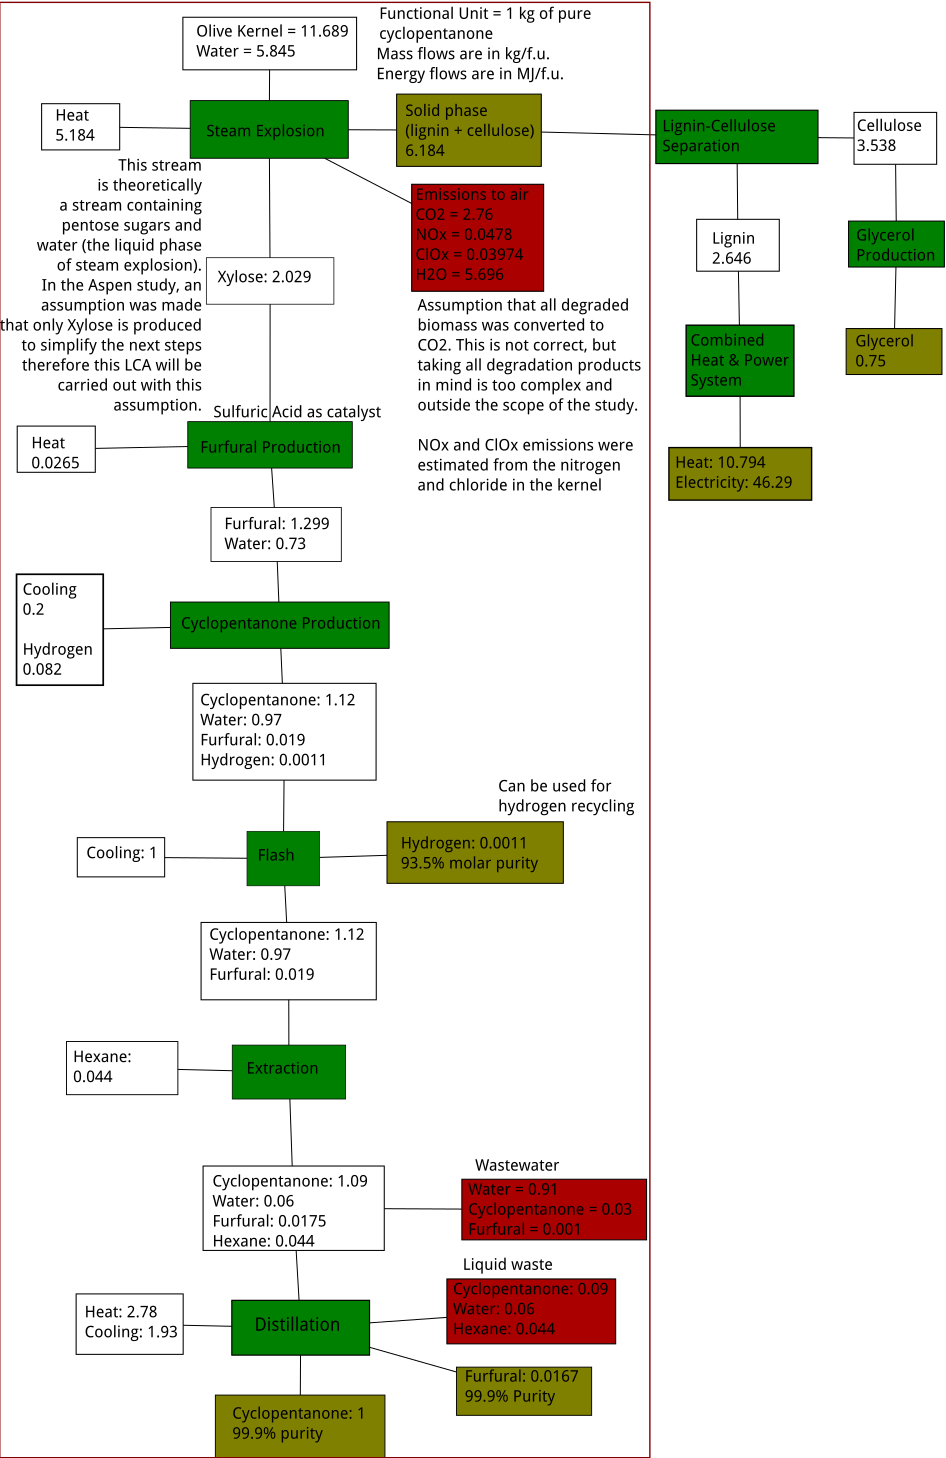
\includegraphics[width=.9\linewidth]{./lca_flowsheet.png}
\end{center}
\pagebreak
\section{Life Cycle Inventory}
\label{sec:org522067a}
\begin{table}[htbp]
\caption{Life Cycle Inventory of the process}
\centering
\begin{tabular}{llrr}
\hline
Stages & Materials & Input (kg/f.u.) & Output (kg/f.u.)\\[0pt]
\hline
Steam Explosion & Olive Kernel & 11.7 & \\[0pt]
 & Xylose &  & 2.03\\[0pt]
 & Solids &  & 6.18\\[0pt]
 & Steam &  & 5.70\\[0pt]
 & CO\textsubscript{2} eq (heat) &  & 0.018\\[0pt]
 & Water & 5.85 & \\[0pt]
 & CO2 &  & 2.76\\[0pt]
 & NO2 &  & 0.048\\[0pt]
\hline
Furfural Production & Xylose & 2.03 & \\[0pt]
 & Furfural &  & 2.03\\[0pt]
 & CO\textsubscript{2} eq (heat) &  & 8.84e-5\\[0pt]
\hline
Cyclopentanone Production & Hydrogen & 0.082 & \\[0pt]
 & Furfural & 2.03 & \\[0pt]
 & Cyclopentanone &  & 2.11\\[0pt]
\hline
Flash & Water & 5 & \\[0pt]
 & Cyclopentanone & 2.11 & 2.11\\[0pt]
 & Hydrogen &  & 0.027\\[0pt]
\hline
Extraction & Hexane & 0.044 & \\[0pt]
 & Cyclopentanone & 2.11 & 1.21\\[0pt]
 & COD &  & 0.076\\[0pt]
\hline
Distillation & Water & 9 & \\[0pt]
 & Cyclopentanone & 1.21 & 1\\[0pt]
 & CO\textsubscript{2} eq (heat) &  & 0.01\\[0pt]
 & COD &  & 3.54\\[0pt]
 & Furfural &  & 0.00167\\[0pt]
\hline
\end{tabular}
\end{table}

\subsection{Assumptions}
\label{sec:org8b74ad5}
To model this process in CCalc, some assumptions were necessary, which are listed below:

\begin{itemize}
\item For cooling needs, tap water is used and no additional energy requirements are listed.
\item For furfural production, catalytic amount of sulfuric acid is used, which isn't included in the LCI
\item The waste streams containing organic compounds (furfural, cyclopentanone, hexane) are assessed cumulatively as Chemical Oxygen Demand, which in CCalc is reflected only in the eutrophication impact.
\item The vapor stream of the Flash is considered pure enough in hydrogen to be a co-product and not a waste material
\item The electricity requirements of the pumps is negligible, while other electricity needs of the factory were not assessed due to difficulty in finding them.
\item Olive kernel was modelled as residual wood chopping.
\item Heat was modelled as Heat at cogen 1400 kWh, wood as in the original aspen, heat was produced from lignin.
\end{itemize}
\subsection{Allocations}
\label{sec:org977201f}
Besides the final product of cyclopentanone, some other streams were considered co-product streams and should somehow be included in the impact assessment. These streams are: The solid stream of steam explosion, which contains cellulose and lignin, the hydrogen rich stream of the flash and the furfural rich stream of the distillation process.

For the first stream, it is hard to assess the economic value of the three components of the kernel (hemicellulose, cellulose and lignin) to do economic allocation and energy allocation isn't very useful, therefore, the allocation methodology followed is mass allocation. The other two streams are very low in quantity and therefore impacts should be allocated to them with mass allocation.

\subsection{Conventional Process LCI}
\label{sec:orgb805191}
For modelling cyclopentanone production in CCalc, Ba(OH)2 was not found in the ecoinvent database, so its production from the mineral barite was modelled based on a patent describing the process [2].

\begin{figure}[htbp]
\centering
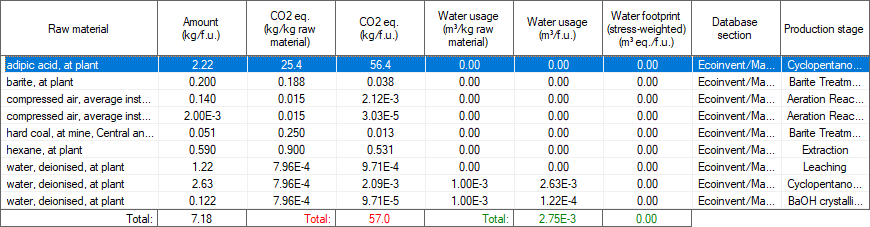
\includegraphics[width=.9\linewidth]{Life_Cycle_Inventory/2024-01-06_15-07-24_screenshot.png}
\caption{LCI of the conventional process}
\end{figure}

Energy data: 2 MJ/f.u. heat (modelled as heavy fuel oil), 2.2 MJ/f.u. electricity (electricity mix, Greece), 0.92 MJ/f.u. cooling (water)

Emissions: 0.075 kg CO2/f.u., 0.048 kg SO2/f.u., 2.1 kg COD/f.u.

\section{Life Cycle Impact Assessment}
\label{sec:org1ef6281}
Modelling the LCI of our process in CCalc, we get the following impacts:

\begin{table}[htbp]
\caption{Impact assessment of our process}
\centering
\begin{tabular}{lr}
Impact Category & Assessment\\[0pt]
\hline
carbon footprint & 0.370\\[0pt]
water usage & 0.020\\[0pt]
energy demand & 34.1\\[0pt]
eutrophication & 0.017\\[0pt]
human toxicity & 0.380\\[0pt]
\end{tabular}
\end{table}

\subsection{Uncertainty analysis}
\label{sec:org3357572}
However, these results have a high amount of uncertainty because much of the LCI was built on assumptions and old data. An uncertainty analysis is important to quantify what our error range is for this process. Furthermore, this analysis can show us what improvement we can expect if we improve one of these parameters. Specifically, from the input variables of the system, we assume quantifiable uncertainty in these:

\begin{itemize}
\item The olive kernel is highly uncertain because data for the steam explosion was taken from literature from 20 years ago. In these years, yields could have significantly improved. Furthermore, an assumption was made that all the sugars in the hemicellulosic stream are xylose which slightly improves the yields we get.
\item The water used for steam explosion is based on a process on a much smaller scale and a linear scale-up was assumed. In reality, the analogy of olive kernel to water might be different.
\item The amount of hexane selected for extraction was arbitrarily calculated in Aspen Plus and gives good results, but is not necessarily optimal.
\item Similarly, the distillation columns are potentially not optimally designed and seeing how changes in them will affect the LCIA is interesting.
\item Lastly, the hydrogen needed might have uncertainty. The data was taken from more recent literature, so we believe its uncertainty is much less than the rest. However, another useful thing assuming uncertainty in hydrogen gives us is that we can see the effect of using less grey hydrogen if the hydrogen is potentially replaced by one produced by a greener technology.

By controlling these 6 design variables (which are not only where we have uncertainty, but also where we have degrees of freedom for improvement) we can see how the process changes. To find the sensitivity of the process in each of these variables, we selected 5 values for each of the variables and ran the LCIA varying each one independently. Some of them, like the olive kernel, also directly causes changes to other parameters, such as the water used for steam explosion (assuming the same analogy), the emissions of the steam explosion process and the solids produced.

With this logic, 30 different simulations were ran. We noticed that the input variables we are controlling are linearly related with the output variables (impacts) and so linear regression was ran to find this exact relation. Since the relation is linear, performing sensitivity analysis of the process is very easy as the sensitivity to each parameter is simply its coefficient in the linear equation.

In the table below, the values of each variable that were used in the simulation are shown.
\end{itemize}

\begin{table}[htbp]
\caption{Uncertainty ranges of each variable}
\centering
\begin{tabular}{rrrrrr}
Olive Kernel & Water & Hexane & Heating & Cooling & Hydrogen\\[0pt]
\hline
6 & 3 & 0.02 & 1.5 & 0.5 & 0.04\\[0pt]
8 & 4 & 0.03 & 2 & 1 & 0.06\\[0pt]
10 & 5 & 0.04 & 2.5 & 1.5 & 0.07\\[0pt]
14 & 7 & 0.08 & 3.5 & 2.5 & 0.09\\[0pt]
16 & 8 & 0.1 & 5 & 4 & 0.1\\[0pt]
\end{tabular}
\end{table}

\subsubsection{Results}
\label{sec:orgc5409ff}
The resulting linear equations correlating input with output are shown below:

\begin{enumerate}
\item Carbon Footprint
\label{sec:org08318c0}
All 6 input variables are correlated with carbon footprint. The corresponding equation is

CF = 0.0109*OK + 0.0084*W + 0.889*HEX + 0.0034*HEAT + 0.0017*COOL + 1.698*H + 0.0022 with R\textsuperscript{2} = 0.987

\item Water Usage
\label{sec:org42d46e4}
Water usage was significantly correlated only with the water used for the steam explosion and the cooling water of the distillation columns with the equation

WU = 0.001*W + 0.00519*COOL + 0.00412 with R\textsuperscript{2} = 0.998

\item Energy Demand
\label{sec:orgb5cc58a}
Energy demand was associated with every input variable with the equation

ED = 0.234*OK + 3.117*W + 61.868*HEX + 1.413*HEAT + 0.0235*COOL + 68.867*H + 0.509 with R\textsuperscript{2} = 0.989

\item Eutrophication
\label{sec:orgab08526}
Eutrophication was correlated only with olive kernel and hexane. Moreover, the impact of the olive kernel is very slight. The equation is:

EP = 0.000582*OK + 0.0833*HEX + 0.0067 with R\textsuperscript{2} = 0.97

\item Human Toxicity
\label{sec:org2307b0a}
Lastly, human toxicity was correlated with all parameters with the equation

HT = 0.0106*OK + 0.03*W + 0.749*HEX + 0.0136*HEAT + 0.00088*COOL + 0.0021*H + 0.00654 with R\textsuperscript{2} = 0.99

\item Range of each impact
\label{sec:org057dacc}
From these equations, we can find the minimum and maximum value of each impact, which allows us to see the range in which the output is, compared to the range of the input.

\begin{table}[htbp]
\caption{Range of the impacts in the uncertainty}
\centering
\begin{tabular}{lrr}
Impact & Minimum & Maximum\\[0pt]
\hline
Carbon Footprint & 0.185 & 0.527\\[0pt]
Water Usage & 0.0097 & 0.0329\\[0pt]
Energy Demand & 17.389 & 49.426\\[0pt]
Eutrophication Potential & 0.0119 & 0.0235\\[0pt]
Human Toxicity & 0.196 & 0.562\\[0pt]
\end{tabular}
\end{table}
\end{enumerate}

\subsubsection{Sensitivity and Hot Spot Analysis}
\label{sec:orge44ec63}
Having seen how the uncertainty of the input affects the uncertainty of the output in a reasonably large domain, we now have a good metric of the sensitivity of the output to each input variable, which shows us what impacts the process most. However, this is not enough. We also need to see the hot spot of each process to see how much of an improvement each variable can truly cause. The diagrams shown below are indicators of these two metrics and allow us to make conclusions for what impacts the process the most and how it could be improved.

\begin{figure}[htbp]
\centering
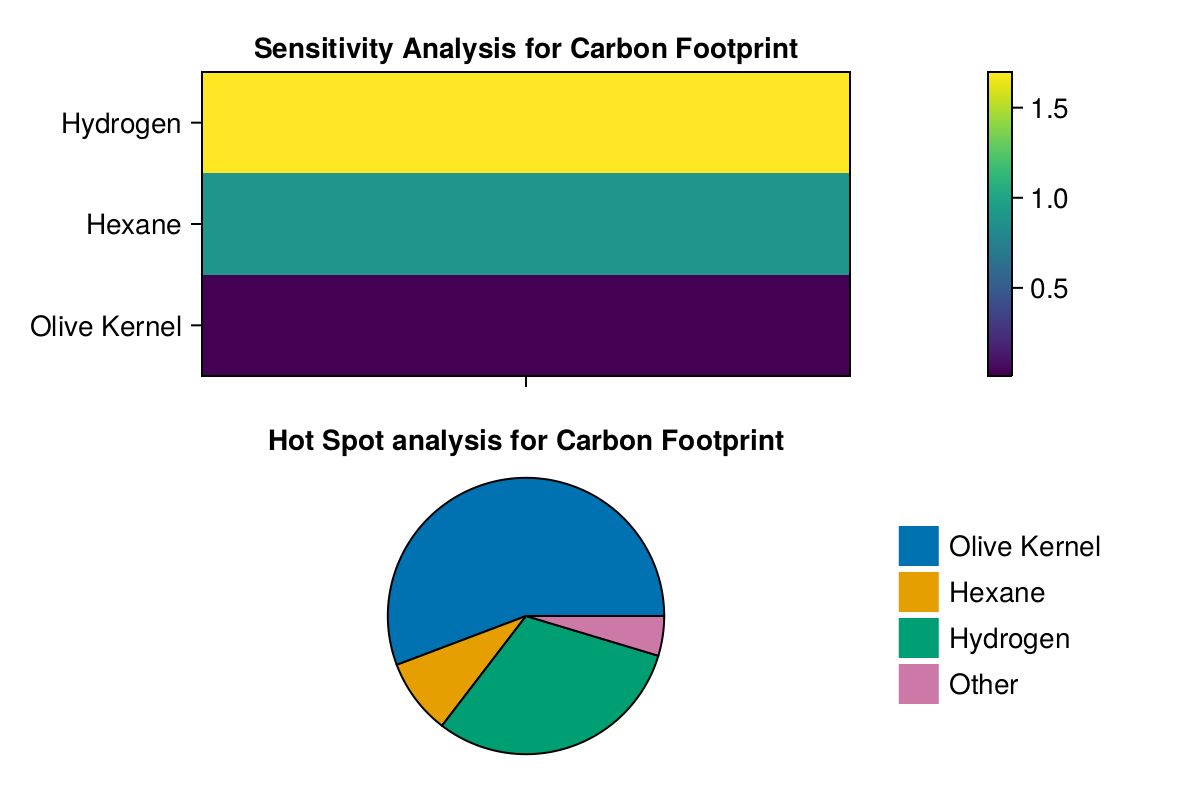
\includegraphics[width=.75\linewidth]{./plots/cf_plots.png}
\caption{Sensitivity and Hot Spot analysis for Carbon Footprint}
\end{figure}

\begin{figure}[htbp]
\centering
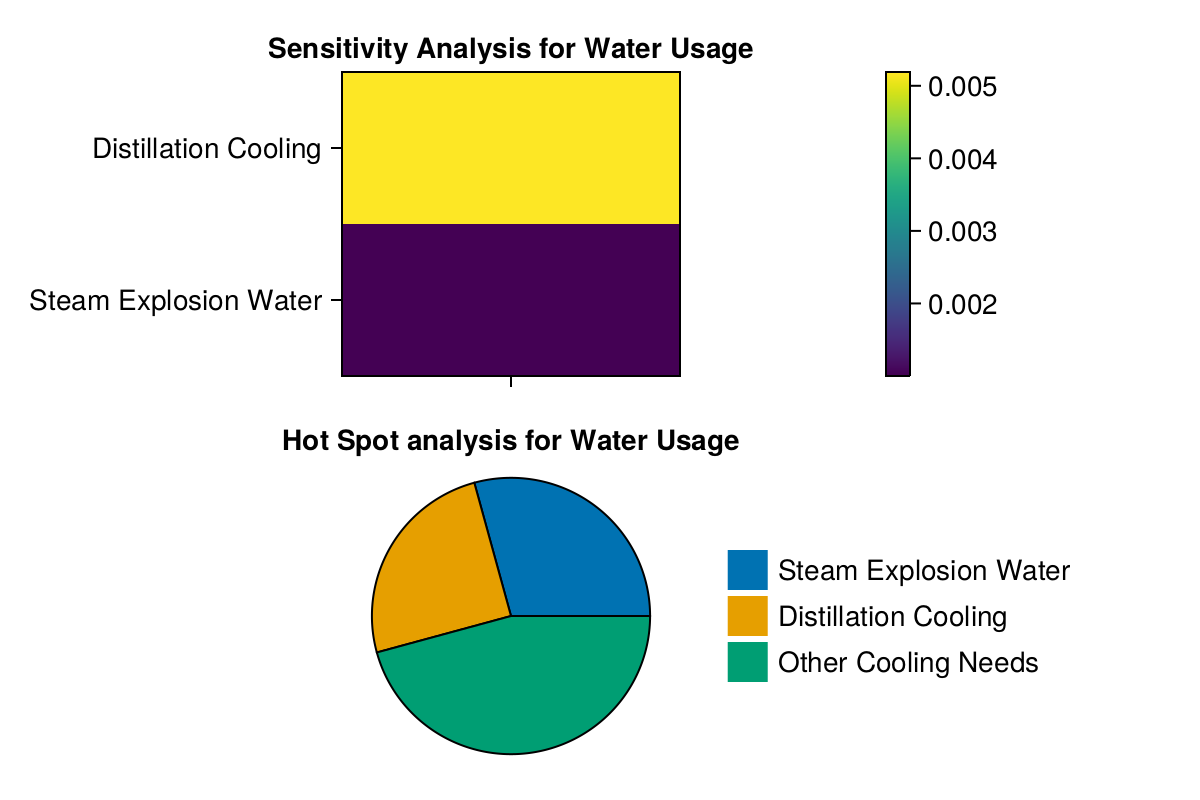
\includegraphics[width=.75\linewidth]{./plots/wu_plots.png}
\caption{Sensitivity and Hot Spot analysis for Water Usage}
\end{figure}

\begin{figure}[htbp]
\centering
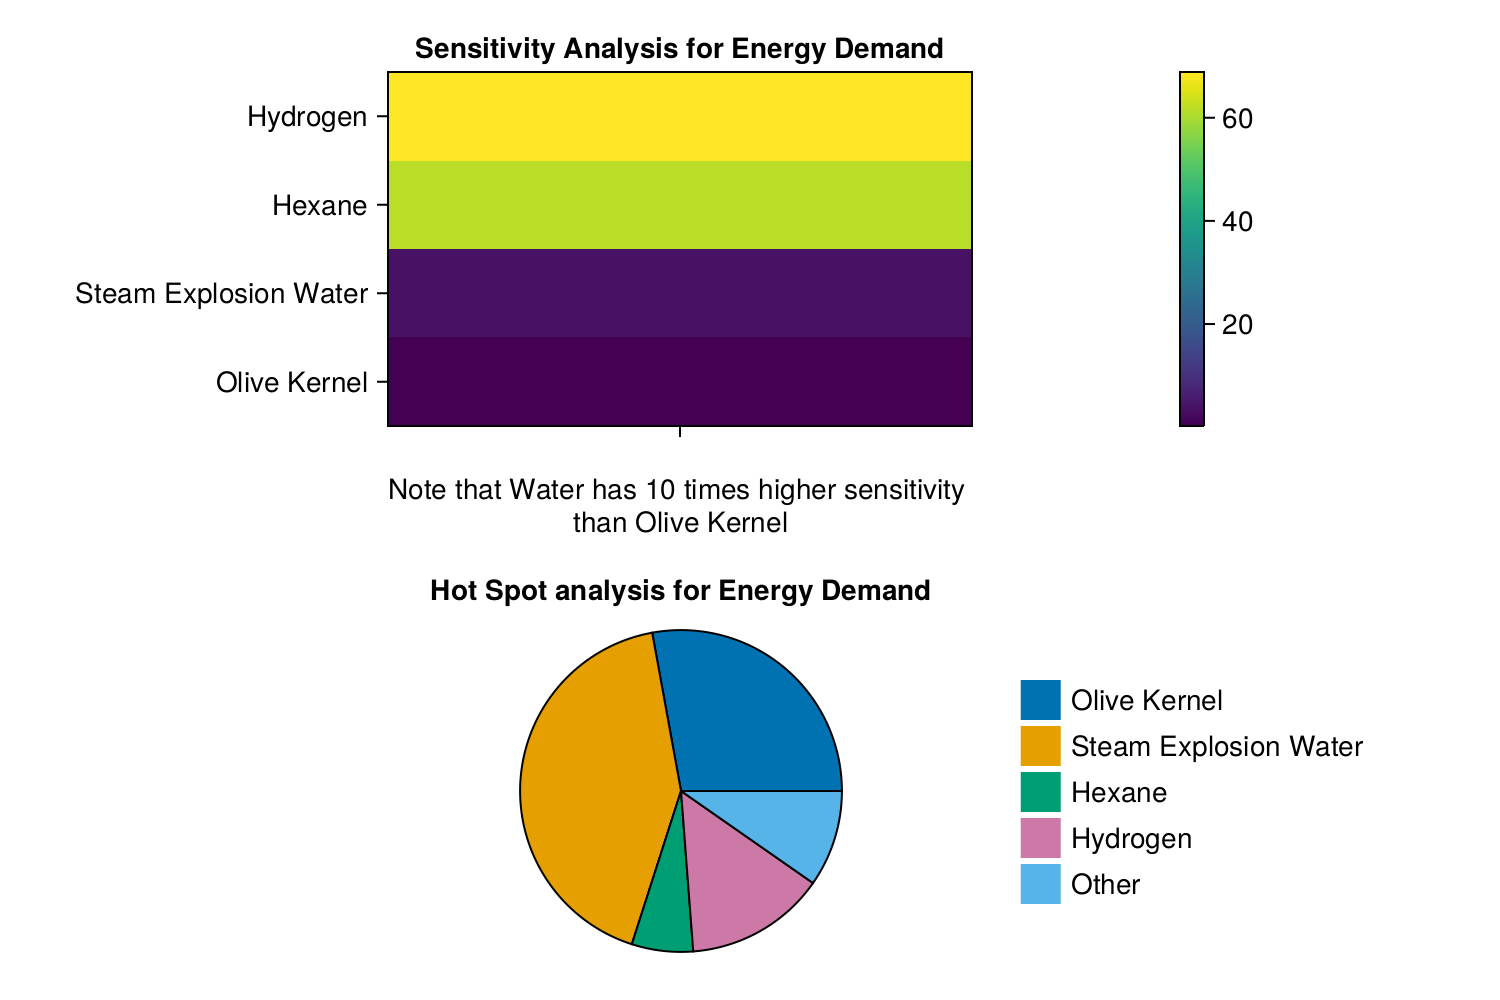
\includegraphics[width=.9\linewidth]{./plots/ed_plots.png}
\caption{Sensitivity and Hot Spot analysis for Energy Demand}
\end{figure}

\begin{figure}[htbp]
\centering
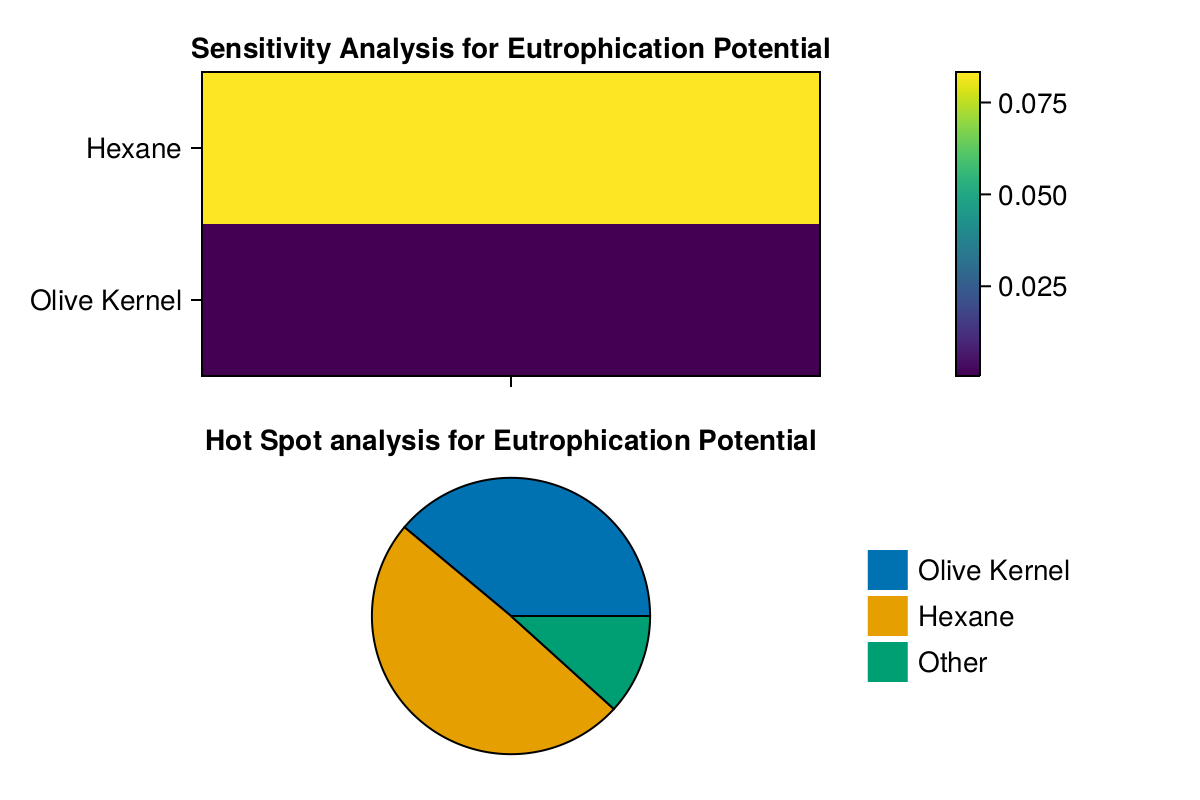
\includegraphics[width=.9\linewidth]{./plots/ep_plots.png}
\caption{Sensitivity and Hot Spot analysis for Eutrophication Potential}
\end{figure}

\begin{figure}[htbp]
\centering
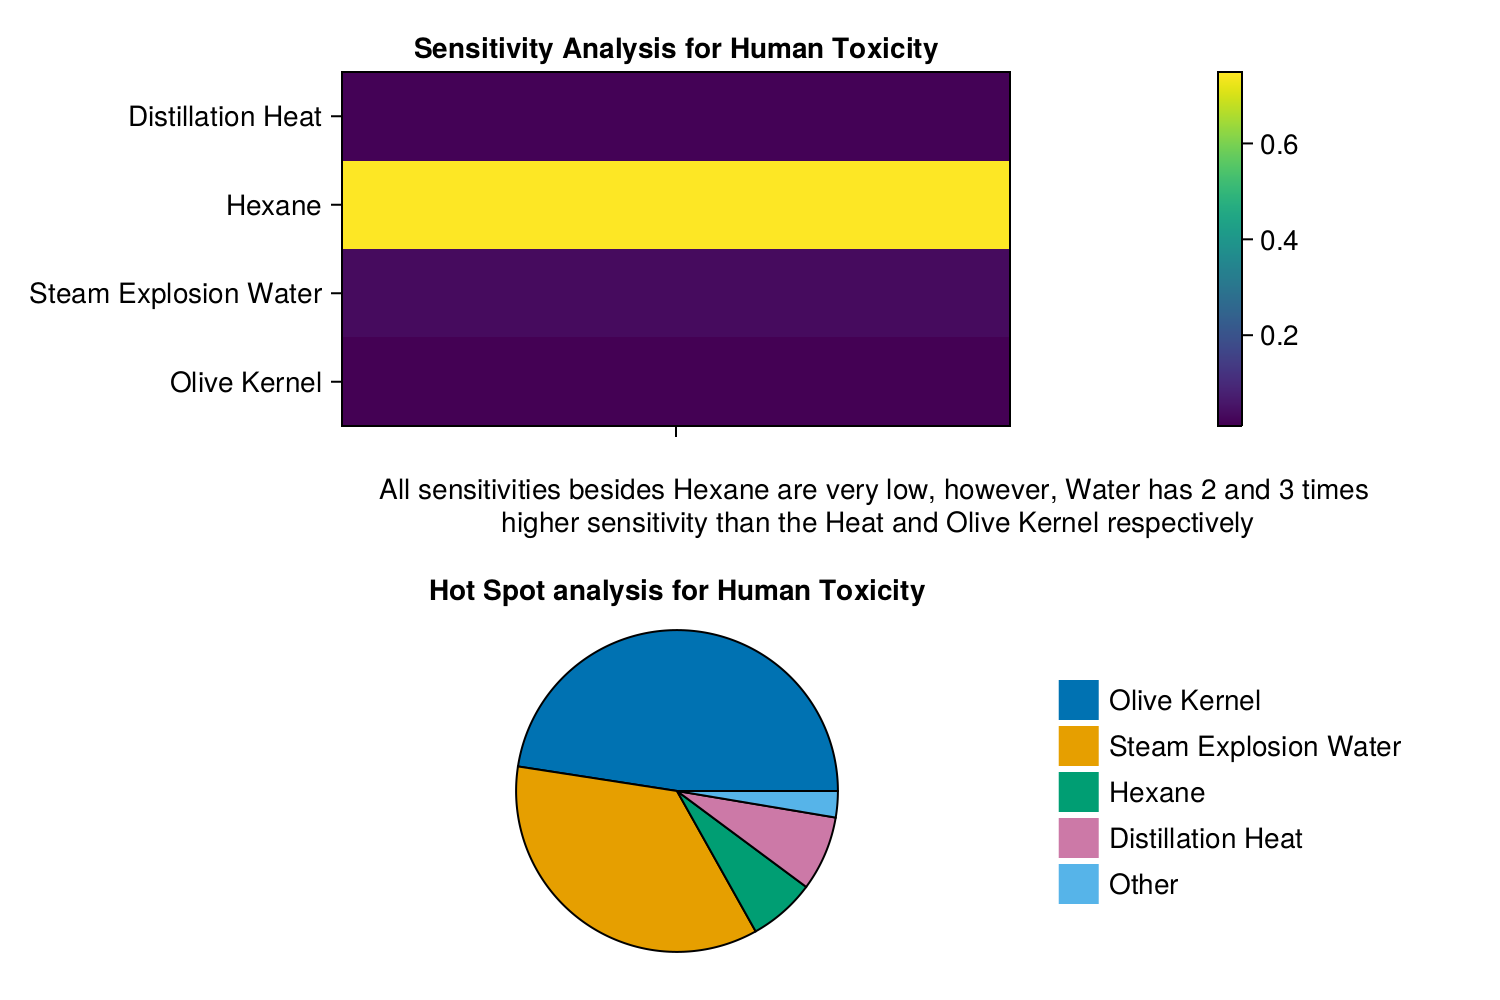
\includegraphics[width=.9\linewidth]{./plots/ht_plots.png}
\caption{Sensitivity and Hot Spot analysis for Human Toxicity}
\end{figure}

\pagebreak

\subsection{Comparison}
\label{sec:orga0be043}
Having seen the LCIA of our process, we can now compare it with the petrelaic process. The diagram shown below, shows the comparative value of each impact for the two processes. Moreover, it lists the worst possible scenario of the biomass process based on the uncertainty analysis.

\begin{figure}[htbp]
\centering
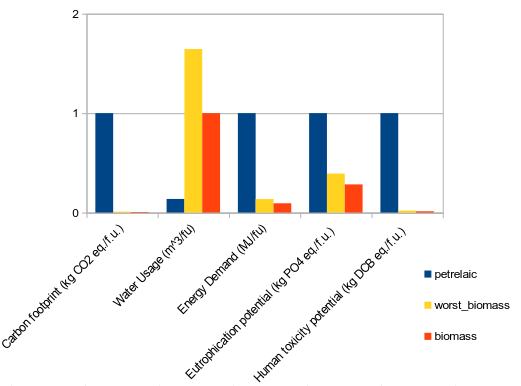
\includegraphics[width=.6\linewidth]{Life_Cycle_Impact_Assessment/2024-01-06_16-23-27_screenshot.png}
\caption{Comparative LCIA of the two processes}
\end{figure}

\pagebreak

We see that our process significantly outperforms the petrelaic one in all sectors besides water usage and that even in the worst scenario included in our uncertainty analysis, this conclusion does not change.

\subsection{Scenario with Water Reuse}
\label{sec:orgf0af253}
Since we saw that water usage is the major problem of the process, we decided to investigate whether or not it is worth to integrate a refrigerator cycle in the process. Its use will be to cover the cooling needs of the distillation columns (which was shown to have the most impact in water usage) but using water that is in the refrigerator cycle and thus not consumed. This will significantly lower the water usage needs. Depending on the design, it might increase energy needs, due to the electricity needed to run the cycle, but by integrating the distillation columns in the cycle, it might decrease the total energy demand. And even if it increases, this area is not the worst part about the proposed process. Below is a graph showing the comparative LCIA of the two processes.

\begin{figure}[htbp]
\centering
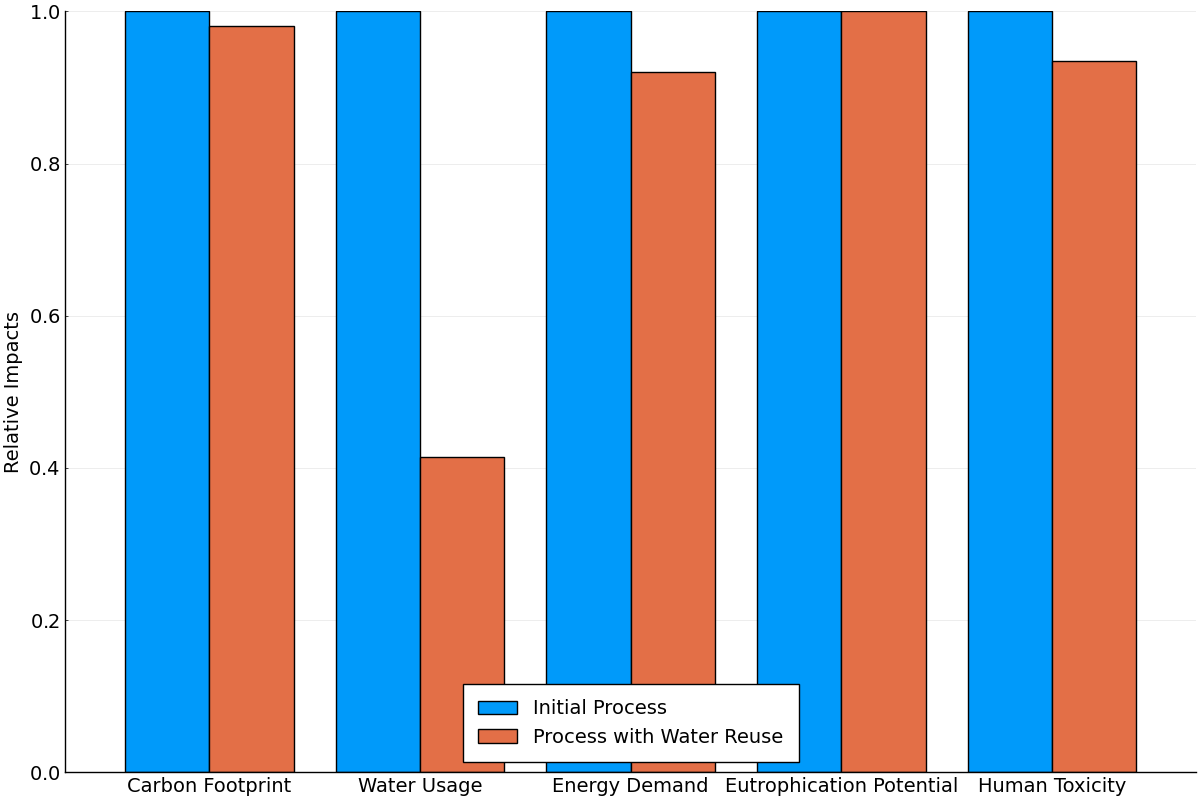
\includegraphics[width=.9\linewidth]{./lcia_comparison_reuse.png}
\caption{Comparative LCIA of the process with and without water reuse}
\end{figure}

It can be seen that water usage becomes 0.4 of its original value, while the carbon footprint, energy demand and human toxicity are slightly reduced, indicating that environmentally, this integration is worth the effort. However, there are some important tradeoffs. Firstly, the energy demand seems lower, but we need energy of higher quality in this equilibrium (electricity instead of heat), which may make the process more expensive. However, due to the assumption we are working under that the plant has a cogeneration system using the lignin of the olive kernel, we can safely assume that the electricity necessary is equivalently available to the heat. This will however lower the income of the plant, which will be able to sell less electricity as a co-product. Moreover, investing in this refrigeration cycle will have a cost for the equipment and especially the compressor of the process, which is an expensive piece of equipment. Due to these two economic concerns, a techno-economic analysis would need to be done to judge whether the decreased environmental impact makes up for the increased cost, but it definitely looks like an interesting proposal.

\subsubsection{Reusing the other cooling water}
\label{sec:org5b6d4fa}
Besides the cooling water of the distillation columns, the other water usage that could be saved with reuse is the cooling right after the reactors. Due to this cooling being at a lower temperature (30 \(^oC\)), it would force the evaporator temperature to be very low, which makes the usage of water hard. The first thought is to try and integrate this stream in the above refrigerating cycle. To do this however, we need a different material for cooling as water cannot achieve such a wide range. The easiest option is \(CH_3Cl\), which would allow us to lower water usage further. However, chloromethane is a health and environmental hazard and we believe that it will be environmentally taxing to change water in our cycle with chloromethane if the goal is to reduce the environmental impacts.

The other option is to use a second refrigerator cycle for this and use the R-134 refrigerant. It is less toxic that chloromethane, but has a higher environmental impact than water. Furthermore, introducing a second refrigerator cycle starts making the economic problems more adverse. A second compressor is necessary and even more energy will need to be supplied to the process. We studied this scenario and found that it was feasible, however, we believe that its economic impact combined with that of the above cycle is almost certain to push our process in a more unfavourable range.

\section{Conclusions}
\label{sec:org2e12368}
We conclude that the proposed process is an environmentally friendly process for producing cyclopentanone from a waste material (olive kernel), which can effectively replace cyclopentanone production from adipic acid, which is very bad both for the environment and for the health of anyone in the factory producing that material.

Furthermore, due to the sensitivity and hot spot analysis performed, we can also assess how the process can be improved.

The biggest problem of the process is water usage. The scenario mentioned above including the refrigeration cycle solves this to an extent. Further integration attempts for other cooling needs of the process, may help even further, so despite this increasing the cost of the process, it is definitely the way forward for decreasing the process water usage.

The second most important parameter is decreasing the amount of olive kernel necessary for the process as it will help in almost all impacts. It is the hot spot of the carbon footprint and human toxicity and plays a role in energy demand and eutrophication potential of the process. The process is not so sensitive to this change as it is to others, but the extraction of xylose from the kernel is highly inefficient and improving that process has potential to significantly decrease the olive kernel requirements and as such lower these impacts.

Decreasing the amount of steam needed for the steam explosion is also very impactful. This will be decreased by decreasing the olive kernel, but if we can find that less water than what was initially assumed (half of the kernel's mass) can be used, this will significantly improve the energy demand of the process (as it is sensitive to it and it is the hot spot of the process), it will improve the human toxicity of the process decently and also lower water usage, albeit it not being the most impactful parameter for this.

Using less hydrogen is the other parameter that can significantly affect the system. It plays a very significant role in the carbon footprint of the process and is the parameter to which the system is the most sensitive to. Decreasing the amount of hydrogen used is rather hard, but replacing the gray hydrogen with something like green hydrogen has the potential of improving the carbon footprint of the process significantly.

Hexane is a parameter to which the system is very sensitive, showing that if we wrongly underestimated its value, we have wrongly assessed the process as much more environmentally friendly than it is. However, for improving the process, there is a very narrow range to which hexane can help, as the amount used is already very low and isn't a significant hot spot. It should be mentioned that decreasing it will lower the eutrophication potential by a wide margin, but the process already has a rather low eutrophication potential so this isn't as significant.

Improving the distillation column design was shown to be the least significant of the parameters used. As mentioned above, it can help the water usage of the process, but besides that, it has a very low impact on everything else.

\section{Bibliography}
\label{sec:org8ec07e1}
[1] Thorpe, J. F., and G. A. R. Kon. “CYCLOPENTANONE.” Organic Syntheses 5 (1925): 37. \url{https://doi.org/10.15227/orgsyn.005.0037}.
[2] Rohrborn, Hans-Joachim. Process for producing barium hydroxide. United States US4060585A, filed February 20, 1976, and issued November 29, 1977. \url{https://patents.google.com/patent/US4060585A/en}.
\end{document}